\documentclass[revision-guide.tex]{subfiles}
% !TEX = xelatex
%% Current Author:
\setcounter{chapter}{19}
\begin{document}
\raggedbottom
\chapter{Astronomy and cosmology}
\begin{content}
    \item standard candles
    \item stellar radii
    \item Hubble's law
    \item the Big Bang theory
    \item the age of the Universe
\end{content}
\spec{understand the terms luminosity and luminous flux}
\spec{recall and use the inverse square law for flux
\begin{equation}
  F = \frac{L}{4\pi d^2}
\end{equation}
}

Stars are described as LUMINOUS because they emit electromagnetic waves.

The LUMINOSITY of a luminous (``hot'') object is defined as the amount
of electromagnetic wave energy emitted by the object per second i.e. it
is the emission Power of the object and is thus measured in Watts (W).
It is a measure of the absolute ``brightness'' of the object.

FLUX (F) is Power per unit area (an Intensity). For a spherical emitter
of radius R (and thus surface area of $ 4\pi R^{2}$), this
means that $F = \frac{L}{4\pi d^2}$.

\spec{understand the need to use standard candles to help determine distances to galaxies}

Standard Candles are types of stars or galaxies for which the Luminosity
(the absolute brightness) can be determined directly from observations.
By measuring the observed brightness and comparing it to the absolute
brightness of the object, it is possible to determine how far away that
object is.

The best-known and most widely used Standard Candles are Cepheid
Variables and Type 1a Supernovae.

Cepheid Variables (named after the star Delta Cephei) pulsate and vary
in brightness with a frequency that is related to the star's Luminosity.
The periods of some Cepheids have been measured as a few days, others a
few months. Once the absolute brightness has been found from the
observed period of the pulsation, it can be compared with the brightness
the star appears to have as observed from the Earth and hence the
distance can be determined.

Type 1a supernovae occur when one of the stars (a white dwarf) in a
binary system gains mass, becomes unstable and catastrophically explodes
emitting vast quantities of light and other electromagnetic energy in
the process. The maximum absolute brightness achieved is related to the
rate at which the emission fades (the so-called Light Curve). Thus,
again, once the absolute brightness is known, a comparison with how
bright the object appears to be from the Earth will yield its distance.
Because they are so bright, these objects can be easily seen in distant
galaxies, so that distances well beyond the limits of the Milky Way can
be established.
\spec{recognise and use Wien's displacement law
\begin{equation}
  \lambda_{\text{max}} \propto  \frac{1}{T}
\end{equation}
to estimate the peak surface temperature of a star either graphically or algebraically}

Black bodies of a particular temperature T will emit radiation over a
range of wavelengths (a radiation distribution known as a Planck Curve):

\begin{figure}[h]
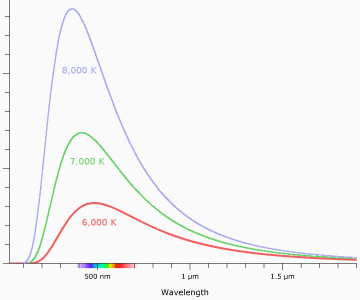
\includegraphics{figs/chapt-20/media/image1.png}
\caption{Planck curves}
\label{plank-curves}
\end{figure}

The distribution peaks at a wavelength λ\textsubscript{max} which is
determined by the reciprocal of the absolute temperature T of the
object. This is known as Wien's Displacement Law. The constant of
proportionality has a value of 2.90 x 10\textsuperscript{-3} m K:

\[\lambda_{max} = \frac{2.90 \times 10^{-3}} {T}\]

The greater the temperature, the larger the area under the curve,
suggesting that more radiation is being emitted altogether, consistent
with the Stefan-Boltzmann relation. Refer to Figure \ref{plank-curves} and consider the T
= 8000 K and the T = 6000 K graphs. The area beneath the T = 8000 K
graph is (8000/6000)\textsuperscript{4} times that beneath the T = 6000
K graph, i.e. 3.16 times greater.

The Sun's photosphere is at a temperature of a little under 6000 K;
notice that the Planck Curve for this temperature peaks at a wavelength
lying in the visible part of the electromagnetic spectrum.

Wien's Displacement Law enables astronomers to determine the temperature
of a star from observations of the light (and other radiation) emitted
by that star.
\spec{recognise and use Stefan's law for a spherical body
\begin{equation}
  L = 4\pi \sigma r^2 T^4
\end{equation}
}

The Stefan-Boltzmann Law (sometimes simply called Stefan's Law) states
that the Flux from a hot object is proportional to the fourth power of
the absolute temperature, T. Strictly speaking, this applies only to
idealised radiation emitters (referred to as ``black bodies''); the
constant of proportionality is the Stefan-Boltzmann constant, $\sigma$, which
has a value of 5.67 x 10\textsuperscript{-8} W m\textsuperscript{-2}
K\textsuperscript{-4}:

\[F = \sigma T^{4}\]

Therefore, for an emitted with surface area A, the Luminosity will be
given by

\[L =\sigma A T^{4}\]

and in the case of a spherical emitter (such as a star) of radius R,
this becomes

\[L = 4 \pi R^{2} \sigma T^{4}\]

\spec{use Wien's displacement law and Stefan’s law to estimate the radius of a star}



Having determined the temperature, T, one can then use the
Stefan-Boltzmann relation to determine the Luminosity, L. This is a
measure of the actual amount of radiation being emitted by the star. By
measuring the actual amount of radiation received per second per unit
area (i.e. the flux, F), one can then calculate how big the star must be
(the surface area from which the radiation is being emitted) in order to
produce that amount of Flux.

\begin{example}
\emph{Worked example: Proxima Centauri, the nearest star to the Sun}

Data:

Parallax angle = 0.8 seconds of arc

Peak wavelength, λ\textsubscript{max} = 967 nm

Flux measured at Earth = 3.56 x 10\textsuperscript{11} W
m\textsuperscript{-2}

\begin{enumerate}
\def\labelenumi{\arabic{enumi}.}
\item
  Calculate the distance to Proxima Centauri.
\item
  Calculate its surface temperature.
\item
  Calculate the Flux at the star's surface
\item
  Hence calculate the radius of the star.
\end{enumerate}

\answer

\begin{enumerate}
\def\labelenumi{\arabic{enumi}.}
\item
  D (in parsecs) = 1 / angle of parallax in seconds of arc = 1.25 pc =
  \emph{3.85 x 10\textsuperscript{16} m}
\item
  From Wien's Displacement Law, T = 2.90 x 10\textsuperscript{-3} m K /
  967 x 10\textsuperscript{-9} m = 3000 K
\item
  From Stefan's Law, F = $\sigma$ T\textsuperscript{4} = 5.67 x
  10\textsuperscript{-8} x 8.10 x 10\textsuperscript{13} = \emph{4.6 x
  10\textsuperscript{6} W m\textsuperscript{-2}}
\item
  Flux measured at a distance of 3.85 x 10\textsuperscript{16} m is 3.56
  x 10\textsuperscript{-11} W m\textsuperscript{-2}.

  So, F\textsubscript{at Earth} / F\textsubscript{star's surface} =.
  (radius of star)\textsuperscript{2} / (distance to
  star)\textsuperscript{2}
\end{enumerate}

\begin{itemize}
\item
  Radius of star = \emph{1.07 x 10\textsuperscript{8} m}
\end{itemize}

\end{example}

\spec{understand that the successful application of Newtonian mechanics and gravitation to the Solar System and beyond indicated that the laws of physics apply universally and not just on Earth}

Newton's law of Universal Gravitation states that two masses, M and m,
whose centres are separated by a distance r, will mutually attract with
a gravitational force given by

\[F = \frac{G M m }{ r^{2}}\]

where G, the Universal Gravitational Constant, = 6.67 x
10\textsuperscript{-11} N m\textsuperscript{2} kg\textsuperscript{-2}.

One of the great triumphs of the law was to demonstrate consistency with
Kepler's Laws of Planetary Motion, formulated empirically some 70 years
earlier. Kepler's Laws state that the planets move about the Sun in
elliptical orbits and whilst Newton's Law can be applied to such orbits,
for simplicity we consider a planet moving in a circular orbit. If the
radius of the orbit is r, then from rotational mechanics, the planet
will experience a constant centripetal force of $mv^{2}/r$.
This origin of this force is the gravitational attraction given by
Newton's equation and by equating the two formulae it is possible to
show that

\begin{equation}
T^{2} = \frac{4 \pi^{2} r^{3}}{ G M}
\end{equation}

i.e. that T\textsuperscript{2} α r\textsuperscript{3} as stated by
Kepler's 3\textsuperscript{rd} Law. Newton's Law, when combined with his
Laws of Motion, was applied to other objects observed to be in
gravitational orbits with great success. The movements of planetary
satellites, binary star systems, galactic spiral arms and even clusters
of galaxies themselves have all been shown to be consistent with the
relationships. Famously, the relationships demonstrated orbital
irregularities in the motion of the planet Uranus, high led to the
discovery of the planet Neptune beyond it. Similar anomalous behaviour
in the rotations of spiral galaxies observed by Vera Rubin has led to
the speculation of the existence of Dark Matter.

\begin{example}

From the orbital data for the Earth, calculate the mass of the Sun
(assuming a circular orbit).

\answer

Radius of Earth's orbit = 150 x 10\textsuperscript{6} km

Orbital period of earth = 1 year = 3.2 x 10\textsuperscript{7} s

\begin{itemize}
\item
  From Kepler's 3\textsuperscript{rd} Law (above), \emph{M = 1.96 x
  10\textsuperscript{30} kg}
\end{itemize}

\end{example}
\spec{recognise and use
\begin{equation}
  \frac{\Delta \lambda}{\lambda} \approx \frac{\Delta f}{f} \approx \frac{v}{c}
\end{equation}
 for a source of electromagnetic radiation moving relative to an observer}

 When a source of waves moves away from an observer (in a stationary
 medium), the observer will receive waves of a longer wavelength (and
 thus lower frequency) than those emitted by the source. If the source
 moves towards the observer then the observed wavelength is shorter
 (frequency is higher). This is called Doppler Shift. For example, with
 sound waves this can be perceived as a change in the pitch of the
 emitted sound.

 The greater the speed of the source, v, the greater the change in the
 wavelength $\Delta \lambda$ (or frequency, $\Delta f$, whichever is being measured) of the
 waves received by the observer in which c is the velocity of the emitted waves (a relationship strictly
 only true for if c is much greater than v).

 The dark lines observed in the visible light spectra of stars and
 galaxies are caused by the absorption of specific frequencies (colours)
 by elements present in those objects, enabling astronomers to determine
 their composition. In the 1920s, Edwin Hubble discovered that the
 absorption lines for distant galaxies were shifted towards the red end
 of the colour (emission) spectrum. This Red Shift indicated that the
 galaxies were moving away (receding) from the Earth. But there were two
 particular features of his discovery that made a special impact:

 \begin{enumerate}
 \def\labelenumi{\alph{enumi})}
 \item
   Galaxies were receding in all directions.
 \item
   The more distant the galaxy, the higher its recessional velocity.
 \end{enumerate}

 (The distances to the galaxies were established using Standard Candles,
 especially Cepheid Variables.)

\spec{state Hubble's law and explain why galactic redshift leads to the idea that the Universe is expanding and to the Big Bang theory}

These observations have led to the conclusion that the universe began
with a Big Bang and what Hubble observed was the expansion of space
itself. A helpful picture is that of the infinite scaffolding by M C
Escher (Figure \ref{mcescher}):

\begin{figure}[h]
\begin{center}
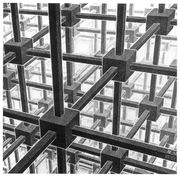
\includegraphics{figs/chapt-20/media/image2.jpeg}
\end{center}
\caption{M C Escher drawing}
\label{mcescher}
\end{figure}

No matter which junction you view from, if each scaffold pole is
expanding, junctions in all directions will appear to recede. Note that,
in effect, the junctions themselves do not move: the space in between
them does. Also, more distant junctions (with more expanding poles
between them and the observer) will appear to recede with greater
speeds.

In such a model, the speed of ``recession'' (expansion) is proportional
to the distance of the observed galaxy and observations are by and large
consistent with this:

$ V = H_{o} d$

in which the constant of proportionality, H\textsubscript{o,} is known
as the Hubble Constant, the value of the gradient of the graph of v
plotted against d (Figure \ref{hubble-law}):

\begin{figure}[h]
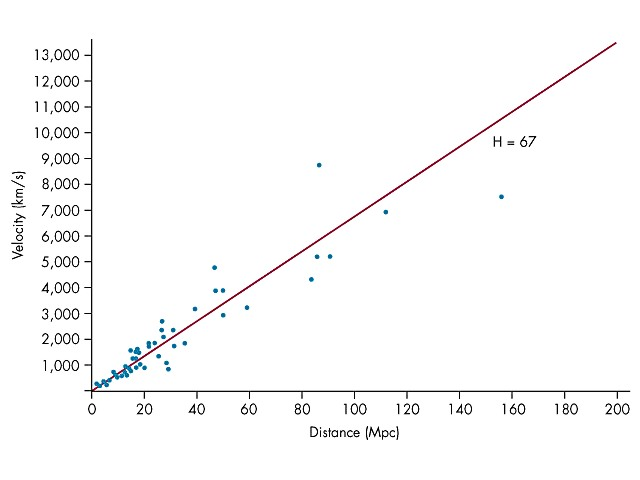
\includegraphics[width=\textwidth]{figs/chapt-20/media/image3.jpeg}
\caption{Hubble's Law}
\label{hubble-law}
\end{figure}

Recent measurements (see graph) suggest a value of H\textsubscript{o} of
a little over 67 km s\textsuperscript{-1} Mpc\textsuperscript{-1}

Given that, in the observable universe, the greatest distance from which
radiation could be received is given by the speed of light x the age of
the universe, it follows that the age of the universe will be given by
1/H\textsubscript{o}. For the value of H\textsubscript{o} quoted, this
equates to an age of

When measuring the red shifts of distant galaxies, the calculated
velocities thus more properly indicate the rate at which the intervening
space is stretching. The value of Δλ/λ (or Δf/f) is called the
Cosmological Red Shift, z, indicating that the space has expanded by a
factor of 1 + z in order to produce the observed Doppler Shift.


The quasar 3C273 was the first object of its kind to be identified. So
called because they were star-like but much more luminous
(``quasi-stellar objects'') they are now known to consist of
supermassive black holes that draw in a huge disc of orbiting gas,
causing large emissions of radiation across a wide range of wavelengths.
Their spectra exhibit large red shifts.


\begin{example}

\begin{enumerate}
\def\labelenumi{\arabic{enumi}.}
\item
  One emission line in the spectrum of 3C273 appears at a wavelength of
  475.0 nm; in the laboratory the same line is measured at 410.2 nm.
  Calculate the recessional velocity of the quasar.
\item
  Using the value of H\textsubscript{0} quoted above, hence calculate
  the distance of 3C273.
\end{enumerate}

\answer

\begin{enumerate}
\def\labelenumi{\arabic{enumi}.}
\item
  Δλ = 475.0 -- 410.2 nm = 64.8 nm.
\end{enumerate}

From Doppler equation, Δλ/λ = v/c, this gives v = 4.74 x
10\textsuperscript{7} ms\textsuperscript{-1} or \emph{4.74 x
10\textsuperscript{4} km s\textsuperscript{-1}}.

\begin{enumerate}
\def\labelenumi{\arabic{enumi}.}
\item
  Assume a value of H\textsubscript{0} of 67 km s\textsuperscript{-1}
  Mpc\textsuperscript{-1}.
\end{enumerate}

\begin{itemize}
\item
  d = 4.74 x 10\textsuperscript{4} km s\textsuperscript{-1} / 67 km
  s\textsuperscript{-1} Mpc\textsuperscript{-1} = \emph{707 Mpc.}
\end{itemize}


\end{example}
\spec{explain how microwave background radiation provides empirical support for the Big Bang theory}
\spec{understand that the theory of the expanding Universe involves the expansion of space-time and does not imply a pre-existing empty space into which this expansion takes place or a time prior to the Big Bang}
\spec{recall and use the equation
\begin{equation}
  v \approx H_0 d
\end{equation}
for objects at cosmological distances}
\spec{derive an estimate for the age of the Universe by recalling and using the Hubble time
\begin{equation}
  t = \frac{1}{H_0}
\end{equation}
}
In the 1940s, George Gamow suggested that the observed ratio of hydrogen
to helium in the universe could be explained by assuming the universe
was much hotter and denser a long time ago, consistent with the idea of
a Big Bang origin stemming from Hubble's work. His theory predicted the
existence of a ``leftover'' radiation which was eventually discovered by
chance in 1965. This is today known as the Cosmic Microwave Background
Radiation and it has the biggest cosmological red shift. It was produced
when the early universe had cooled down to about 3000K, low enough for
electrons to combine with protons to produce atoms, a process resulting
in the emission of photons of wavelengths around 1 mm. Because of
cosmological expansion, the wavelength is now a thousand times bigger
(millimetres) and the temperature a thousand times smaller, about 3 K.

Refinements to the Big Bang model have included a period of Inflation
very early on which gave rise to the eventual clumping of matter, which
accounts for the later existence of stars and galaxies (and planets and
humans). The Cosmic Background Explorer satellite revealed such clumping
(measured as tiny temperature fluctuations in the background radiation)
and further evidence is still being sought to confirm Inflation as a
part of the model.

\begin{figure}[h]
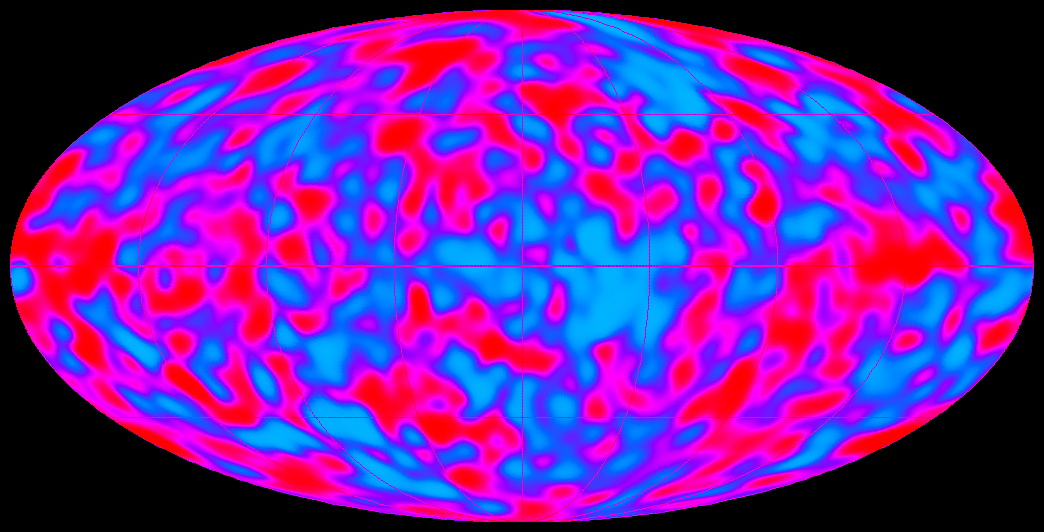
\includegraphics[width=\textwidth]{figs/chapt-20/media/image4.jpeg}
\caption{COBE satellite image}
\end{figure}
\end{document}
